\chapter{Recursive Data Types}\label{recursive_data_chapter}

\subsubsection{Substituting into Aexp's}
Substituting expressions for variables is a standard, important
operation.  For example the result of substituting the expression $3x$ for $x$
in the $(x(x-1))$ would be $(3x(3x-1)$.  We'll use the general
notation $\msubst{f}{e}$ for the result of substituting an $\aexp$, $f$,
for each of the $x$'s in an $\aexp$, $e$.  For instance,
\[
\msubst{3x}{x(x-1)} = 3x(3x-1).
\]

This substitution function has a simple recursive definition:

\begin{definition}\label{subst-def}
  The \term{substitution function} from $\aexp \times \aexp$ to \aexp\ is
  defined recursively on expressions, $e \in \aexp$, as follows.  Let $f$
  be any $\aexp$.

\begin{itemize}
\item \textbf{Base cases:}

\begin{enumerate}

\item\label{subst-var} Case[$e$ is $x$]
\[
\msubst{f}{x} \eqdef f.
\]
(The result of substituting $f$ for the variable, $x$, is just $f$.)

\item\label{subst-const} Case[$e$ is $\mtt{k}$]
\[
\msubst{f}{\mtt{k}} \eqdef \mtt{k}.
\]
(The numeral, $\mtt{k}$, has no $x$'s in it to substitute for.)

\end{enumerate}

\item \textbf{Constructor cases:}

\begin{enumerate}
\setcounter{enumi}{2}
\item\label{subst-sum} Case[$e$ is $(e_1 \sumsym e_2)$]
\[
\msubst{f}{(e_1 \sumsym e_2)}) \eqdef  (\msubst{f}{e_1} \sumsym
\msubst{f}{e_2}).
\]

\item\label{subst-prod} Case[$e$ is $(e_1 \prodsym e_2)$]
\[
\msubst{f}{(e_1 \prodsym e_2)}) \eqdef  (\msubst{f}{e_1} \prodsym
\msubst{f}{e_2}).
\]

\item\label{subst-minus} Case[$e$ is $\minussym(e_1)$]
\[
\msubst{f}{\minussym(e_1)} \eqdef \minussym (\msubst{f}{e_1}).
\]

\end{enumerate}
\end{itemize}
\end{definition}

Here's how the recursive definition of the substitution function would find
the result of substituting $3x$ for $x$ in the $x(x-1)$:
\begin{align*}
\msubst{3x}{(x(x-1))} & =
\msubst{3x}{(x \prodsym (x \sumsym \minussym(1)))} & \text{(unabbreviating)}\\
 & = (\msubst{3x}{x} \prodsym \msubst{3x}{(x \sumsym \minussym(1))})
         & \text{(by~Def~\ref{subst-def}~\ref{subst-prod})}\\
 & = (3x \prodsym \msubst{3x}{(x \sumsym \minussym(1))})
         & \text{(by~Def~\ref{subst-def}~\ref{subst-var})}\\
 & = (3x \prodsym (\msubst{3x}{x} \sumsym \msubst{3x}{\minussym(1)}))
         & \text{(by~Def~\ref{subst-def}~\ref{subst-sum})}\\
 & = (3x \prodsym (3x \sumsym \minussym (\msubst{3x}{1})))
         & \text{(by~Def~\ref{subst-def}~\ref{subst-var} \&~\ref{subst-minus})}\\
 & = (3x \prodsym (3x \sumsym \minussym (1)))
         & \text{(by~Def~\ref{subst-def}~\ref{subst-const})}\\
 & = 3x(3x-1) & \text{(abbreviation)}
\end{align*}

Now suppose we have to find the value of $\msubst{3x}{(x(x-1))}$ when $x =
2$.  There are two approaches.

First, we could actually do the substitution above to get $3x(3x-1)$, and
then we could evaluate $3x(3x-1)$ when $x =2$, that is, we could
recursively calculate $\meval(3x(3x-1),2)$ to get the final value 30.  In
programming jargon, this would be called evaluation using the
\emph{Substitution Model}.  Tracing through the steps in the evaluation,
we find that the Substitution Model requires two substitutions for
occurrences of $x$ and 5 integer operations: 3 integer multiplications, 1
integer addition, and 1 integer negative operation.  Note that in this
Substitution Model the multiplication $3 \cdot 2$ was performed twice to
get the value of 6 for each of the two occurrences of $3x$.

The other approach is called evaluation using the \emph{Environment
  Model}.  Namely, we evaluate $3x$ when $x = 2$ using just 1
multiplication to get the value 6.  Then we evaluate $x(x-1)$ when $x$ has
this value 6 to arrive at the value $6\cdot 5=30$.  So the Environment
Model requires 2 variable lookups and only 4 integer operations: 1
multiplication to find the value of $3x$, another multiplication to find
the value $6 \cdot 5$, along with 1 integer addition and 1 integer
negative operation.

So the Environment Model approach of calculating
\[
\meval(x(x-1), \meval(3x,2))
\]
instead of the Substitution Model approach of calculating
\[
\meval(\msubst{3x}{x(x-1)},2)
\]
is faster.  But how do we know that these final values reached by these
two approaches always agree?  We can prove this easily by structural
induction on the definitions of the two approaches.  More precisely, what
we want to prove is

\begin{theorem}\label{environments}
For all expressions $e,f \in \aexp$ and $n \in \integers$,
\begin{equation}\label{eval-subst}
\meval(\msubst{f}{e},n) = \meval(e, \meval(f,n)).
\end{equation}
\end{theorem}

\begin{proof}
The proof is by structural induction on $e$.\footnote{This is an example
of why it's useful to notify the reader what the induction variable is---in this case it isn't $n$.}

\textbf{Base cases:}
\begin{itemize}

\item Case[$e$ is $x$]

  The left hand side of equation~\eqref{eval-subst} equals $\meval(f,n)$
  by this base case in Definition~\ref{subst-def} of the substitution
  function, and the right hand side also equals $\meval(f,n)$ by this base
  case in Definition~\ref{meval-def} of $\meval$.


\item Case[$e$ is $\mtt{k}$].

  The left hand side of equation~\eqref{eval-subst} equals $\mtt{k}$ by
  this base case in Definitions~\ref{subst-def} and~\ref{meval-def} of
  the substitution and evaluation functions.  Likewise, the right hand
  side equals $\mtt{k}$ by two applications of this base case in the
  Definition~\ref{meval-def} of $\meval$.

\end{itemize}

\textbf{Constructor cases}:
\begin{itemize}

\item Case[$e$ is $(e_1 \sumsym e_2)$]

  By the structural induction hypothesis~\eqref{eval-subst}, we may assume
  that for all $f \in \aexp$ and $n \in \integers$,

\begin{equation}\label{ln4.hyp}
\meval(\msubst{f}{e_i},n)  =  \meval(e_i, \meval(f,n))
\end{equation}
for $i= 1,2$.  We wish to prove that

\begin{equation}\label{s+}
\meval(\msubst{f}{(e_1\sumsym e_2)},n)  =  \meval((e_1 \sumsym e_2), \meval(f,n))
\end{equation}

But the left hand side of~(\ref{s+}) equals
\[
\meval(\, (\msubst{f}{e_1} \sumsym \msubst{f}{e_2}),\ n)
\]
by Definition~\ref{subst-def}.\ref{subst-sum} of substitution into a sum
expression.  But this equals
\[
\meval(\msubst{f}{e_1},n) + \meval(\msubst{f}{e_2},n)
\]
by Definition~\ref{meval-def}.\ref{eval-sum} of $\meval$ for a sum expression.  By
induction hypothesis~\eqref{ln4.hyp}, this in turn equals
\[
\meval(e_1,\meval(f,n)) + \meval(e_2,\meval(f,n)).
\]
Finally, this last expression equals the right hand side of~(\ref{s+}) by
Definition~\ref{meval-def}.\ref{eval-sum} of $\meval$ for a sum
expression.  This proves~(\ref{s+}) in this case.

\item $e$ is $(e_1 \prodsym e_2)$.  Similar.

\item $e$ is $-(e_1)$.  Even easier.

\end{itemize}

This covers all the constructor cases, and so completes the proof by
structural induction.

\end{proof}

\begin{editingnotes}

\subsection{A String Theorem}

Here is a more complex proof, illustrating a combination of structural
induction and strengthening the hypothesis.

\begin{theorem}
  In a string of $0$s and $1$s, the number of occurrences of the pattern
  $01$ is less than or equal to the number of occurrences of $10$, plus
  one.
\end{theorem}

Let's try to prove this by structural induction.  First we must
define $P(s)$.  Let's write $\ms{num}(pat,s)$ as the number of
occurrences of the pattern string pat in s.  Now our inductive
hypothesis is
\[
P(s): \ms{num}(01,s) \leq \ms{num}(10,s) + 1. 
\]
If you try to prove this by structural induction, you will get
stuck.
Why? 
Consider what happens when you add $1$ at the end.  
This could increase the number of $01$s without increasing the number of
$10$s. 

So, to prove by structural induction on strings, let's strengthen the
hypothesis by adding another clause.  If a string ends in $0$ then
the number of $01$s is less than or equal to the number of $10$s.
That solves the problem by weakening what we have to show when the
string ends in $1$.  But maybe it causes another problem somewhere
else.  Let's give it a try:

Redefine $P(s) \eqdef$
\begin{eqnarray*}
\ms{num}(01,s) & \leq & \ms{num}(10,s) + 1, \text{ and}\\
\lefteqn{\text{If $s$ ends in $0$ then}}\\
\ms{num}(01,s) & \leq  &\ms{num}(10,s).
\end{eqnarray*} 
 
This means that, for each inductive step have two things to show.
\iffalse

\structuredproof{

  Prove: $\forall s \in S \; (P(s))$ \\
  1. (Base) $P(\emptystring)$ 
  \reason{No patterns of either kind.} \\
  2. (Inductive step) $\forall s \in S \; (P(s) \implies P(s 0))$ \\
  1. Fix $s$. \\
  2. Assume $P(s)$. \\
  3. $P(s 0)$ \\
  1. $\ms{num}(01,s0) \leq \ms{num}(10,s0) + 1$. 
  \reason{???} \\
  2. If $s 0$ ends in $0$ then $\ms{num}(01,s0) \leq
  \ms{num}(10,s0)$. \noreason \\
  \reason{???} \\
  3. QED
  \reason{Conjunction} \\
  4. QED 
  \reason{Implication, UG} \\
  3. (Inductive step) $\forall s \in S \; (P(s) \implies P(s 1))$ \\
  1. Fix $s$. \\
  2. Assume $P(s)$. \\
  3. $P(s 1)$ \\
  1. $\ms{num}(01,s1) \leq \ms{num}(10,s1) + 1$. 
  \reason{???} \\
  2. If $s 1$ ends in $0$ then $\ms{num}(01,s1) \leq
  \ms{num}(10,s1)$.\noreason \\
  \reason{???} \\
  3. QED
  \reason{Conjunction} \\
  4. QED 
  \reason{Implication, UG} \\
  4. QED
  \reason{Structural induction on strings.}\\
}\fi

\textcolor{blue}{Structured proof display commented out here}

First let's consider $s1$. This is the case that looks dangerous,
because it might increase the number of $01$s.  We have to prove two
statements.  The second is easy, because the new string doesn't end in
$0$.  We say it's ``vacuously true''.

The first statement now takes some work. 
We might be adding to the number of $01$s.  
However, if we do, the previous string must have ended with $0$. 
Then the inductive hypothesis says that the previous string had to
satisfy the stronger inequality in the second statement. 
Adding one to the LHS of the stronger inequality yields the weaker
inequality we want.

The following proof fragment considers cases based on whether $s$ ends
in $0$ or not.  If not, it might end in $1$, or might be empty (don't
forget this possibility).

\textcolor{blue}{Structured proof display commented out here}
\iffalse

\begin{proof}
  3. $P(s 1)$ \\
  1. $\ms{num}(01,s1) \leq \ms{num}(10,s1) + 1$. \\
  1. If $s$ ends in $0$ then $\ms{num}(01,s1) \leq\ms{num}(10,s1) + 1$. \\
  1. Assume $s$ ends in $0$. \\
  2. $\ms{num}(01,s) \leq \ms{num}(10,s)$ 
  Inductive hypothesis (3.2), part 2. \\
  3. $\ms{num}(01,s1) = \ms{num}(01,s) + 1$ 
  Adding one more $01$. \\
  4. $\ms{num}(10,s1) = \ms{num}(10,s)$ \\
  5. $\ms{num}(01,s1) \leq\ms{num}(10,s1) + 1$. 
  Algebra (combining 3.3.1.1.2, ...3, and ...4) \\
  QED 
  Implication \\
  2. If $s$ ends in $1$ then $\ms{num}(01,s1)\leq\ms{num}(10,s1) + 1$. \\
  Inductive hypothesis, part 1; no new $01$s. \\
  3. If $s = \emptystring$ then $\ms{num}(01,s1) \leq\ms{num}(10,s1)+ 1$. \\
  $s1$ is just $1$, which has no $01$s. \\
  4. QED 
  Cases \\
  2. If $s 1$ ends in $0$ then $\ms{num}(01,s1) \leq \ms{num}(10,s1)$. \\
  Vacuously true, because $s1$ doesn't end in $0$. \\
  3. QED
  Conjunction \\
\end{proof}
\fi

Of course, you could also expand the step for $s$ ending in $1$ into a
careful series of inequalities.

Now consider $s0$.  We hope that what we did to make the $s1$ case
work doesn't mess up the $s0$ case.  But we have to check.

The first statement is easy.  It follows from the first statement of
the inductive hypothesis for $s$, because we are not increasing the
number of $01$s.  But now the second statement takes more work.  The
difficulty is that the new string ends in $0$, which means that we
have to show the stronger inequality in the second statement.  But to
do this, we might only have the weaker inequality for the previous
string.  The argument again depends on what the previous string $s$
ended with.  So again, we consider cases, based on whether $s$ ends in
$0$ or $1$, or is empty.  If $s$ ends in $0$ we rely on the second
statement of the inductive hypothesis for $s$ (with the stronger
inequality), whereas if $s$ ends in $1$ we rely on the first statement
(with the weaker inequality).  In this case, we have to ``turn the
weaker inequality into the stronger inequality''.

\iffalse
\structuredproof[38ex]{
  3. $P(s 0)$ \\
  1. $\ms{num}(01,s0) \leq \ms{num}(10,s0) + 1$.
  \reason{Induct. hypothesis, part 1; no new $01$s.} \\
  2. If $s 0$ ends in $0$ then $\ms{num}(01,s0) \leq\ms{num}(10,s0)$. \\
  1. $\ms{num}(01,s0) \leq \ms{num}(10,s0)$. \\
  1. If $s$ ends in $0$ then $\ms{num}(01,s0)
  \leq\ms{num}(10,s0)$. \noreason \\
  \reason{Induct. hypothesis, part 2; no new $01$s} \\
  2. If $s$ ends in $1$ then $\ms{num}(01,s0)
  \leq\ms{num}(10,s0)$. \noreason \\ 
  1. Assume $s$ ends in $1$. \\
  2. $\ms{num}(01,s) \leq \ms{num}(10,s) + 1$. 
  \reason{Inductive hypothesis, part 1} \\
  3. $\ms{num}(01,s0) = \ms{num}(01,s)$ \\
  4. $\ms{num}(10,s0) = \ms{num}(10,s) + 1$ 
  \reason{Exactly one new occurrence of $10$.} \\
  5. $\ms{num}(01,s0) \leq \ms{num}(10,s0)$ 
  \reason{Algebra} \\
  6. QED
  \reason{Implication} \\
  3. If $s = \emptystring$ then $\ms{num}(01,s0) \leq
  \ms{num}(10,s0)$. \noreason \\ 
  
\reason{$s0$ is just $1$, which has no $01$s or $10$s.} \\
  4. QED 
  \reason{Cases} \\
  2. QED
  \reason{Propositional reasoning (truth table)} \\
  3. QED 
  \reason{Conjunction}\\
}
\fi

\textcolor{blue}{Structured proof display commented out here}

If you actually write out all these cases in the proof, you will
notice that some facts are stated repeatedly, e.g., that when you add
a $0$ to the end of a string you are not increasing the number of
$01$s.  To avoid having to state these facts several times, you can
move them earlier in the proof.

\end{editingnotes}


\begin{editingnotes}

\begin{example*}
\begin{definition}\label{E}
Define a set, $E$, recursively as follows:
\begin{itemize}
\item \textbf{Base case:} $0 \in E$,\label{0E}
\item \textbf{Constructor cases:} if $n \in E$, then
\begin{enumerate}
\item $n+2 \in E$, when $n\geq 0$;\label{+2E}
\item $-n \in E$, when $n > 0$.\label{-E}
\end{enumerate}
\end{itemize}

\end{definition}
\end{example*}

Using this definition, we can see that $0 \in E$ by the Base case, so $0 +
2 = 2 \in E$ by Constructor case~\ref{+2E}., and so $2+2 =4 \in E$, $4+2 =
6 \in E$, \dots, and in fact any nonnegative even number is in $E$ by
successive application of case~\ref{+2E}.  Also, by case~\ref{-E}.,
$-2,-4,-6,\dots \in E$.  So clearly all the even integers are in $E$.

Is anything else in $E$?  The definition doesn't say so explicitly, but an
implicit condition on a recursive definition is that the only way things
get into $E$ is as a consequence of the Base and Constructor cases.  In
other words, $E$ will be exactly the set of even integers.

A very simple application of structural induction proves that the set $E$
given by Definition~\ref{E} is exactly the set of even numbers.  We already
explained why all the even numbers are in $E$.  So what's left is to show
that:

\begin{lemma*}
Every number in the set $E$ in Definition~\ref{E} is even.
\begin{proof}
The proof is by structural induction on $n \in E$.  The induction
hypothesis is 
\[
Q(n) \eqdef \text{$n$ is even}.
\]

\textbf{Base case}: $Q(0)$ holds since 0 is even.

\textbf{Constructor cases}: assuming $n \in E$ and $Q(n)$ holds, prove
that
\begin{itemize}

\item $Q(n+2)$ holds.  This is immediate, since adding 2 to an even number
  gives an even number.

\item $Q(-n)$ holds.  This is also immediate, since $n$ is even iff $-n$ is
even.

\end{itemize}

This completes the proof of the Constructor cases, and we conclude by
structural induction at $Q(n)$ holds for all $n \in E$.
\end{proof}

\end{lemma*}


defining the set, $E$, of even numbers as in Definitions~\ref{E}, but
without the conditions~\ref{+2E}.\ and~\ref{-E}.\ that restrict application of
the rules.  Namely,

\begin{definition}\label{Eamb}
Define a set, $E'$, recursively as follows:
\begin{itemize}
\item \textbf{Base case:} $0 \in E'$,\label{0Eamb}
\item \textbf{Constructor cases:} if $n \in E'$, then
\begin{enumerate}
\item $n+2 \in E'$, \label{+2Eamb}
\item $-n \in E'$.\label{-Eamb}
\end{enumerate}
\end{itemize}
\end{definition}

Now Definition~\ref{Eamb} is perfectly legitimate, and we could us it to
prove by structural induction that $E'$ also is the set of even integers,
that is, $E'= E$.  But Definition~\ref{Eamb} is ambiguous.  For example,
$0\in E'$ by the base case, but also $0=-0 \in E'$ by applying constructor
case~\ref{-Eamb} to the base case.  This begins to matter when we try to
define a function, $s$, from $E'$ to nonnegative integers based on
Definition~\ref{Eamb}:
\begin{align*}
  s(0) & \eqdef 1,\\
s(n+2) & \eqdef 1+ s(n),\\
 s(-n) & \eqdef 1+ s(n).
\end{align*}
So $s(0) \eqdef 1$ by the base case of this definition, and also $s(0)=
s(-0) \eqdef 1+s(0) = 1 + 1 = 2$ by the second constructor case, which
shows that these rules are inconsistent.

On the other hand, using the unambiguous Definition~\ref{E} of $E$,
essentially the same definition of $S$ works just fine.  Namely, define
\begin{align*}
  s(0) & \eqdef 1,\\
  s(n+2) & \eqdef 1+ s(n), & \text{ for } n \geq 0\\
  s(-n) & \eqdef 1+ s(n) & \text{ for } n > 0.
\end{align*}
Now $s(n)$ is unambiguously defined, and in fact is precisely the (unique)
number of steps required to construct $n \in E$ according to the
unambiguous Definition~\ref{E} of $E$.

\end{editingnotes}


%% Structural Induction on Recursive Data Types
%% Problems %%%%%%%%%%%%%%%%%%%%%%
\begin{problems}

\practiceproblems
\pinput{MQ_ambiguous_recursive-def}

\classproblems
\pinput{CP_F18_functions}
\pinput{CP_recursively_defined_sets}
\pinput{CP_erasable_strings}
\pinput{CP_binary_trees}

\homeworkproblems
\pinput{PS_bracket_good_count}
\pinput{PS_koch_snowflake}

\end{problems}

%% Games as a Recursive Data Type %%%%%%%%%%%%%%%%%%%%%%%%%%%%%%%%%%%%%%%%%%%%%
\section{Games as a Recursive Data Type}

Chess, Checkers, and Tic-Tac-Toe are examples of \emph{two-person
terminating games of perfect information}, ---$\tg$'s for short.  These
are games in which two players alternate moves that depend only on the
visible board position or state of the game.  ``Perfect information''
means that the players know the complete state of the game at each move.
(Most card games are \emph{not} games of perfect information because
neither player can see the other's hand.)  ``Terminating'' means that play
cannot go on forever ---it must end after a finite number of
moves.\footnote{Since board positions can repeat in chess and checkers,
termination is enforced by rules that prevent any position from being
repeated more than a fixed number of times.  So the ``state'' of these
games is the board position \emph{plus} a record of how many times
positions have been reached.}

We will define $\tg$'s \iffalse in a straightforward way tagged\fi as a 
recursive data type.  To see how this will work, let's use the game of
Tic-Tac-Toe as an example.

\subsection{Tic-Tac-Toe}

Tic-Tac-Toe is a game for young children.  There are two players who
alternately write the letters ``X'' and ``O'' in the empty boxes of a $3
\times 3$ grid.  Three copies of the same letter filling a row, column, or
diagonal of the grid is called a \emph{tic-tac-toe}, and the first player
who gets a tic-tac-toe of their letter wins the game.

\begin{editingnotes}
Children generally don't take long to figure out an optimal strategy
for playing the game.
\end{editingnotes}

We're now going give a precise mathematical definition of the Tic-Tac-Toe
\term{game tree} as a recursive data type.
\begin{editingnotes}
Children of course have no need for such a definition, and it would be
too complicated for them anyway.  But if we had to write a Tic-Tac-Toe
playing \emph{computer program}, we'd need this kind of picky
precision.
\end{editingnotes}

Here's the idea behind the definition: at any point in the game, the
``board position'' is the pattern of X's and O's on the $3 \times 3$
grid.  From any such Tic-Tac-Toe pattern, there are a number of next
patterns that might result from a move.  For example, from the initial
empty grid, there are nine possible next patterns, each with a single
X in some grid cell and the other eight cells empty.  From any of
these patterns, there are eight possible next patterns gotten by
placing an O in an empty cell.  These move possibilities are given by
the
game tree for Tic-Tac-Toe indicated in
Figure~\ref{fig:Tic-Tac-Toe}.

\begin{figure}[htbp]
\centering
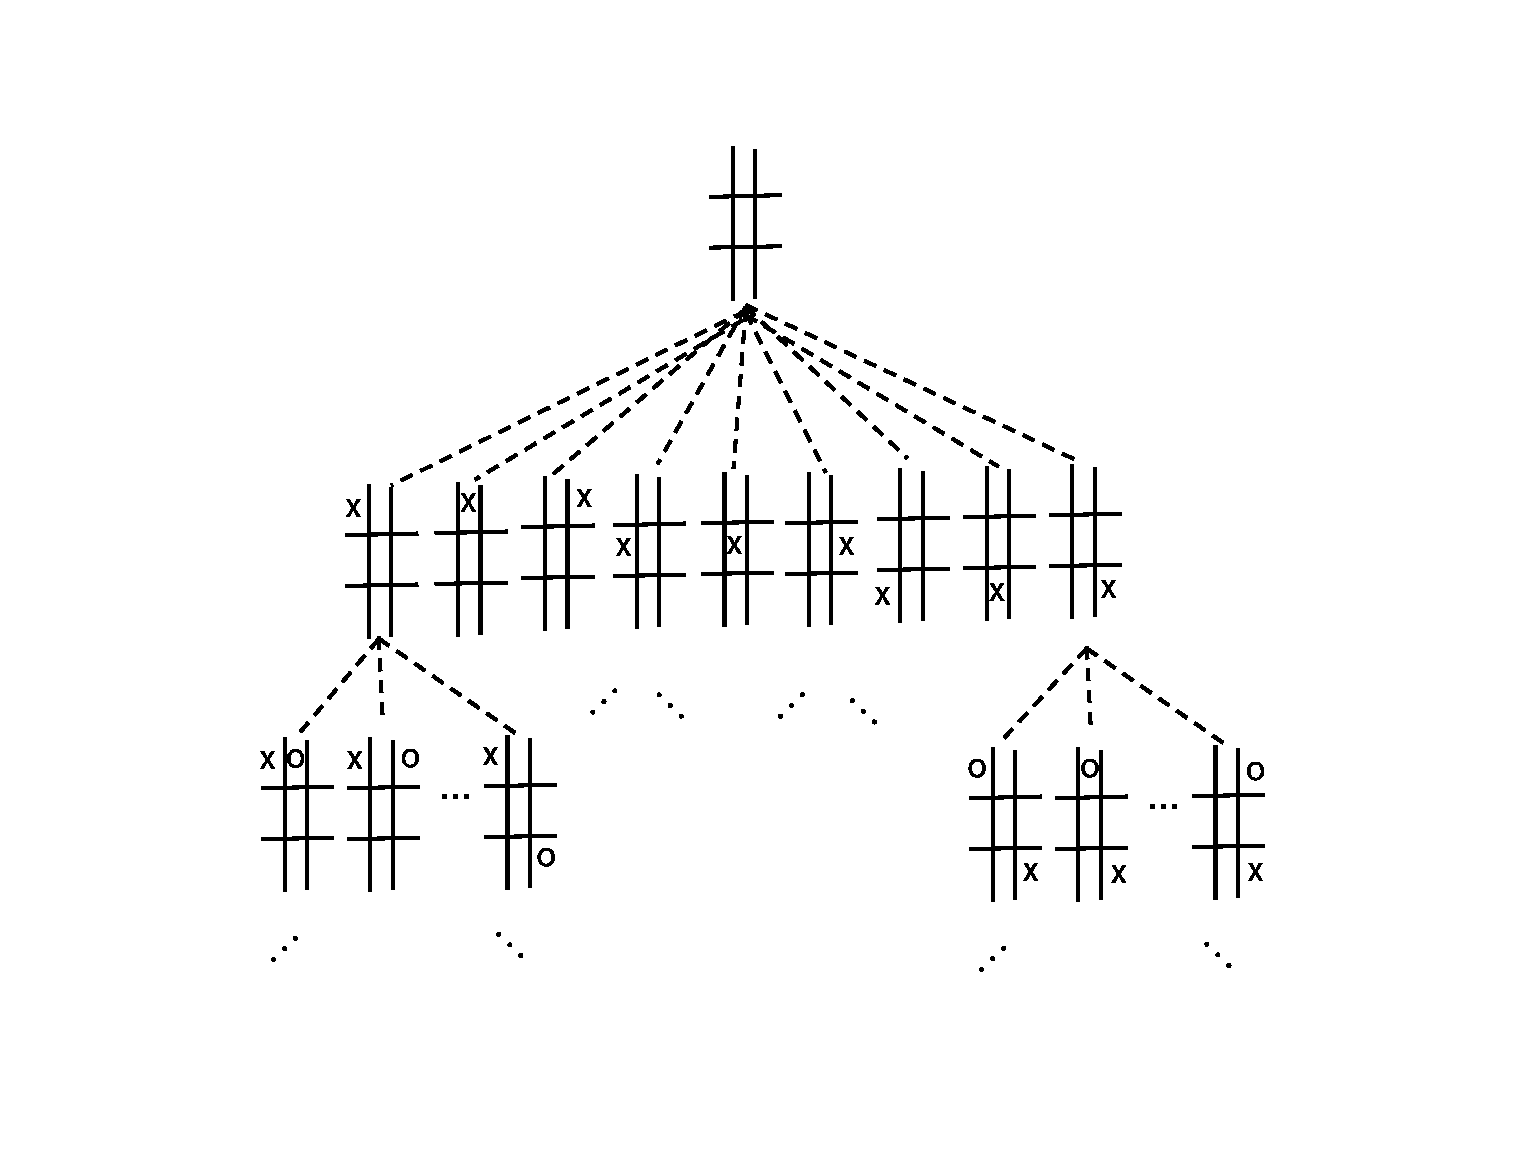
\includegraphics[height=6in]{topgame}
\caption{The Top of the Game Tree for Tic-Tac-Toe.}
\label{fig:Tic-Tac-Toe}
\end{figure}


\iffalse
\[\begin{array}{c|c|c}
\hspace{.1in} & \hspace{.1in} & \hspace{.1in}\\
\hline  & &\\
\hline  & &
\end{array}\]

\textbf{FIGURE NEEDED}
\fi

\begin{definition}

A Tic-Tac-Toe \emph{pattern} is a $3 \times 3$ grid each of whose 9 cells
contains either the single letter, X, the single letter, O, or is
empty.
\begin{editingnotes}

Moreover, there must be either
\begin{itemize}

\item one more X than O's, with at most two tic-tac-toes of X's, and no
tic-tac-toe of O's, or

\item an equal number of X's and O's, with at most one tic-tac-toes of
O's, and no tic-tac-toe of X's.
\end{itemize}

\end{editingnotes}

A pattern, $Q$, is a \emph{possible next pattern after} $P$, providing $P$
has no tic-tac-toes and
\begin{itemize}

\item if $P$ has an equal number of X's and O's, and $Q$ is the same as
$P$ except that a cell that was empty in $P$ has an X in $Q$, or

\item if $P$ has one more X than O's, and $Q$ is the same as $P$ except
that a cell that was empty in $P$ has an O in $Q$.
\end{itemize}

If $P$ is a Tic-Tac-Toe pattern, and $P$ has no next patterns, then the
\emph{terminated Tic-Tac-Toe game trees} at $P$ are

\begin{itemize}

\item 
$\ang{P, \ang{\texttt{win}}}$,
if $P$ has a tic-tac-toe of X's.


\item 
$\ang{P, \ang{\texttt{lose}}}$, if $P$ has a tic-tac-toe of O's.


\item $\ang{P, \ang{\texttt{tie}}}$, otherwise.

\end{itemize}

\iffalse
If $Q$ is a possible move from $P$, then the game tree starting at $Q$ is
called a \emph{  Notice
that $\mathcal{G}_P = \emptyset$ iff $P$ is terminated.}
\fi

The \emph{Tic-Tac-Toe game trees starting at $P$} are defined recursively:

\textbf{Base Case}:
A terminated Tic-Tac-Toe game tree at $P$ is a Tic-Tac-Toe game tree
starting at $P$.

\textbf{Constructor case}: If $P$ is a non-terminated Tic-Tac-Toe pattern,
then the Tic-Tac-Toe game tree starting at $P$ consists of $P$ and the set
of all game trees starting at possible next patterns after $P$.
\end{definition}

For example, if
\begin{align*}
P_0 & =  \begin{array}{c|c|c}
                O & X & O\\
         \hline X & O & X\\
         \hline X & &
        \end{array}\\
Q_1 & = \begin{array}{c|c|c}
                O & X & O\\
         \hline X & O & X\\
         \hline X &  & O
        \end{array}\\
Q_2 & = \begin{array}{c|c|c}
                O & X & O\\
         \hline X & O & X\\
         \hline X & O & 
        \end{array}\\
R & = \begin{array}{c|c|c}
                O & X & O\\
         \hline X & O & X\\
         \hline X & O & X
        \end{array}
\end{align*}
the game tree starting at $P_0$ is pictured in Figure~\ref{fig:endgame}.

\begin{editingnotes}

Then,
\begin{equation}\label{endgame}
\ang{P, \set{\ang{Q_1, \ang{\texttt{lose}}},
             \ang{Q_2, \set{\ang{R,\ang{\texttt{tie}}}}}}}
\end{equation}
is the tagged recursive datum that corresponds to a Tic-Tac-Toe ``end
game'' that starts with $P$.  This game is easier to understand by looking
at its game tree in Figure~\ref{fig:endgame}.  Notice that the game tree
---which so far we haven't actually defined ---is simply the parse tree of
the tagged datum.

\end{editingnotes}

\begin{figure}[htbp]
\centering
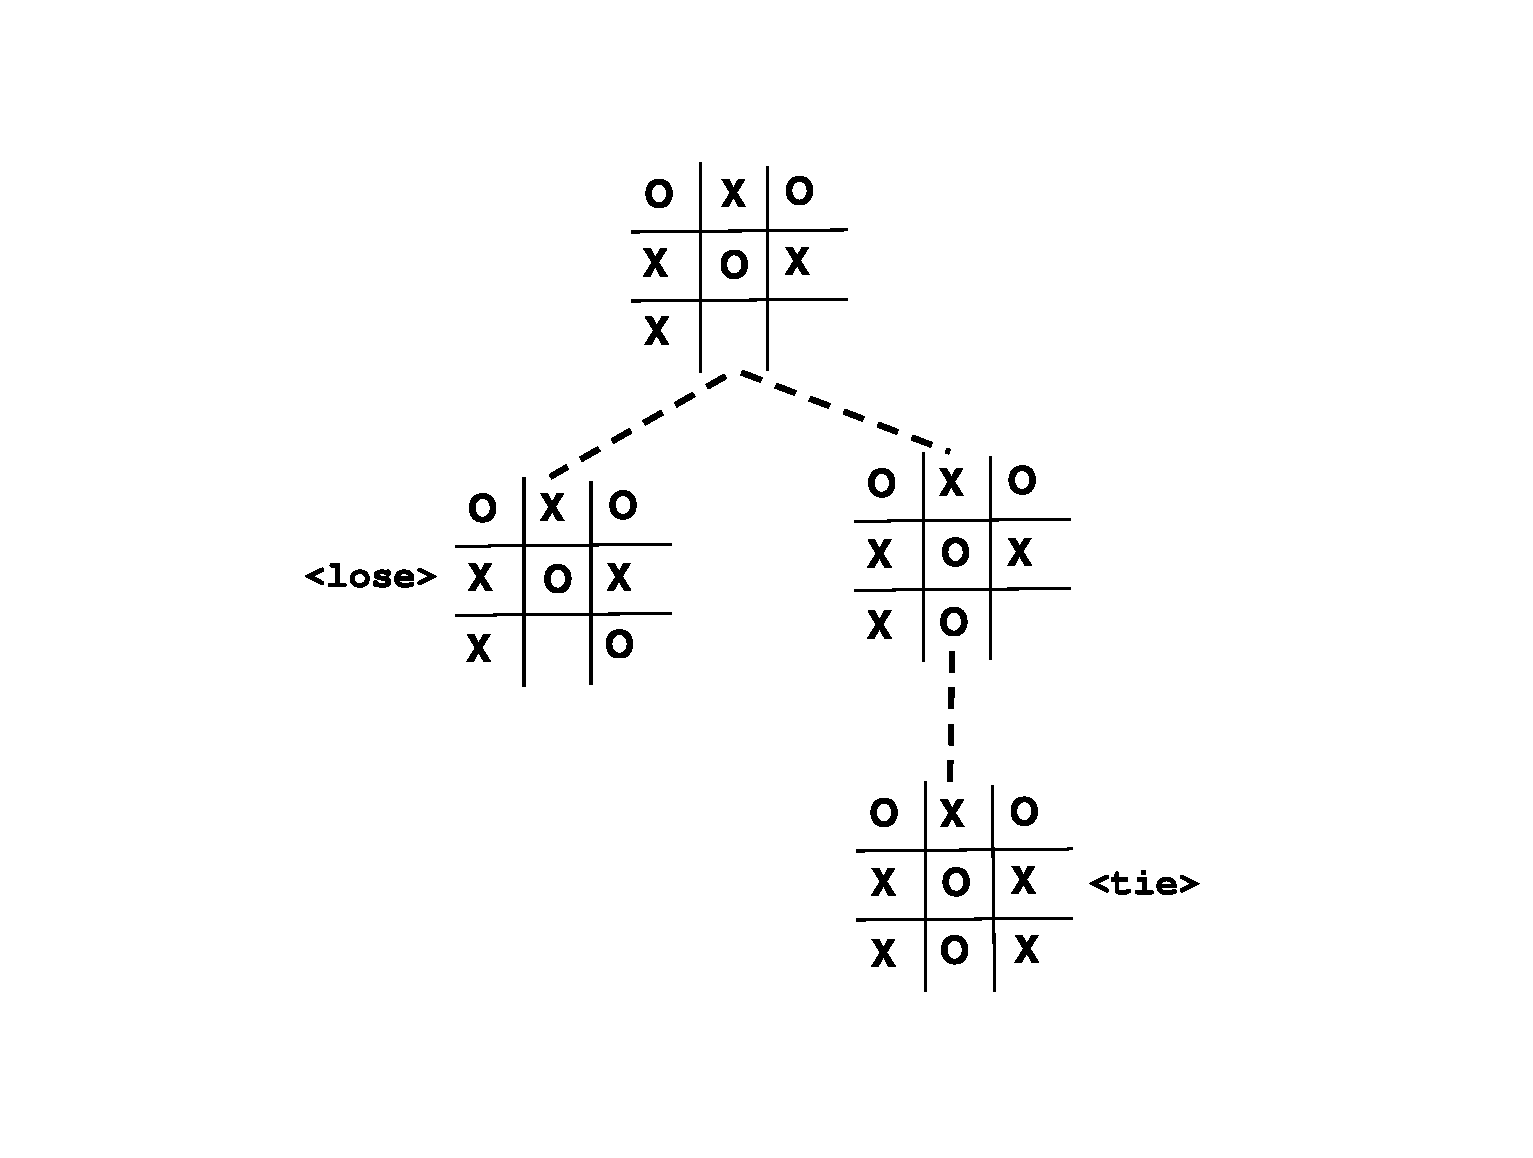
\includegraphics[height=4in]{endgame}
\caption{Game Tree for the Tic-Tac-Toe game starting at $P_0$.}
\label{fig:endgame}
\end{figure}

Game trees are usually pictured in this way with the starting pattern
(referred to as the ``root'' of the tree) at the top and lines connecting
the root to the \iffalse roots of the \fi game trees that start at each
possible next pattern.  The ``leaves'' at the bottom of the tree (trees
grow upside down in computer science) correspond to terminated games.  A
path from the root to a leaf describes a complete \emph{play} of the game.
(In English, ``game'' can be used in two senses: first we can say that
Chess is a game, and second we can play a game of Chess.  The first usage
refers to the data type of Chess game trees, and the second usage refers to
a ``play.'')

\subsection{Infinite Tic-Tac-Toe Games}

At any point in a Tic-Tac-Toe game, there are at most nine possible
next patterns, and no play can continue for more than nine moves.  But
we can expand Tic-Tac-Toe into a larger game by running a 5-game
tournament: play Tic-Tac-Toe five times and the tournament winner is
the player who wins the most individual games.  A 5-game tournament
can run for as many as 45 moves.

It's not much of generalization to have an \emph{$n$-game Tic-Tac-Toe
  tournament}.  But then comes a generalization that sounds simple but can
be mind-boggling: consolidate all these different size tournaments into a
single game we can call \emph{Tournament-Tic-Tac-Toe ($T^4$)}.  The first
player in a game of $T^4$ chooses any integer $n > 0$.  Then the players
play an $n$-game tournament.  Now we can no longer say how long a $T^4$
play can take.  In fact, there are $T^4$ plays that last as long as you
might like: if you want a game that has a play with, say, nine billion
moves, just have the first player choose $n$ equal to one billion.  This
should make it clear the game tree for $T^4$ is infinite.

But still, it's obvious that every possible $T^4$ play will stop.
That's because after the first player chooses a value for $n$, the
game can't continue for more than $9n$ moves.  So it's not possible to
keep playing forever even though the game tree is infinite.

This isn't very hard to understand, but there is an important
difference between any given $n$-game tournament and $T^4$: even
though every play of $T^4$ must come to an end, there is no longer any
initial bound on how many moves it might be before the game ends ---a
play might end after 9 moves, or $9(2001)$ moves, or $9(10^{10}+1)$
moves.  It just can't continue forever.

\begin{editingnotes}

While there is no bound on how long to play, at least after the
first move to an $n \times n$ board in meta-Tic-Tac-Toe, we know the game
will end with $n^2$ moves.

\end{editingnotes}

Now that we recognize $T^4$ as a \tg, we can go on to
a \emph{meta}-$T^4$ game, where the first player chooses a number,
$m>0$, of $T^4$ games to play, and then the second player gets the
first move in each of the individual $T^4$ games to be played.

Then, of course, there's meta-meta-$T^4$\dots.

\begin{editingnotes}
Every play of the meta-meta game must still end, but now even
after the first move, there is no bound on how long a game might
continue.
\end{editingnotes}

\subsection{Two Person Terminating Games}

Familiar games like Tic-Tac-Toe, Checkers, and Chess can all end in
ties, but for simplicity we'll only consider win/lose games ---no
``everybody wins''-type games at MIT.\smiley\ \ But everything we
show about win/lose games will extend easily to games with ties, and
more generally to games with outcomes that have different payoffs.

\begin{editingnotes}

Of course Tic-Tac-Toe and the
other games will fit this set up if we treat a game that ends in a tie as
a loss for the usual first player ---White in Chess, Red in Checkers, the
X-player in Tic-Tac-Toe.

\end{editingnotes}

Like Tic-Tac-Toe, or Tournament-Tic-Tac-Toe, the idea behind the
definition of $\tg$'s as a recursive data type is that making a move
in a $\tg$ leads to the start of a subgame.  In other words, given any
set of games, we can make a new game whose first move is to pick a
game to play from the set.

So what defines a game?  For Tic-Tac-Toe, we used the patterns and the
rules of Tic-Tac-Toe to determine the next patterns.  But once we have
a complete game tree, we don't really need the pattern labels: the
root of a game tree itself can play the role of a ``board position''
with its possible ``next positions'' determined by the roots of its
subtrees.  So any game is defined by its game tree.  This leads to the
following very simple ---perhaps deceptively simple ---general
definition.

\begin{definition}
The $\tg$, \emph{game trees for two-person terminating games of
    perfect information} are defined recursively as follows:
\begin{itemize}

\item \textbf{Base cases:}
\[\begin{array}{ll}
\ang{\texttt{leaf},\texttt{win}} & \in \tg, \text{ and}\\
\ang{\texttt{leaf},\texttt{lose}}& \in \tg.
\end{array}\]

\item \textbf{Constructor case:}
If $\mathcal{G}$ is a nonempty set of
$\tg$'s, then $G$ is a $\tg$, where
\[
G \eqdef \ang{\texttt{tree},\mathcal{G}}.
\]
The game trees in $\mathcal{G}$ are called the possible \emph{next moves}
from $G$.
\end{itemize}

\end{definition}

These games are called ``terminating'' because, even though a $\tg$ may be
a (very) infinite datum like Tournament$^2$-Tic-Tac-Toe, every play of a
$\tg$ must terminate.  This is something we can now prove, after we give a
precise definition of ``play'':

\begin{definition}
A \emph{play} of a $\tg$, $G$, is a (potentially infinite) sequence of
$\tg$'s starting with $G$ and such that if $G_1$ and $G_2$ are consecutive
$\tg$'s in the play, then $G_2$ is a possible next move of $G_1$.

If a $\tg$ has no infinite play, it is called a \emph{terminating} game.
\end{definition}

\begin{theorem}
Every $\tg$ is terminating.
\end{theorem}

\begin{proof}
By structural induction on the definition of a $\tg$, $G$, with induction
hypothesis
\[
G \text{ is terminating}.
\]

\textbf{Base case}: If $G = \ang{\texttt{leaf}, \texttt{win}}$ or $G =
\ang{\texttt{leaf}, \texttt{lose}}$ then the only possible play of $G$ is
the length one sequence consisting of $G$.  Hence $G$ terminates.

\textbf{Constructor case}: For $G = \ang{\texttt{tree},\mathcal{G}}$, we
must show that $G$ is terminating, given the Induction Hypothesis that
\emph{every} $G' \in \mathcal{G}$ is terminating.

But any play of $G$ is, by definition, a sequence starting with $G$ and
followed by a play starting with some $G_0 \in \mathcal{G}$.  But $G_0$ is
terminating, so the play starting at $G_0$ is finite, and hence so is the
play starting at $G$.

This completes the structural induction, proving that every \tg, $G$, is
terminating.
\end{proof}


\subsection{Game Strategies}

A key question about a game is whether a player has a winning strategy.  A
\emph{strategy} for a player in a game specifies which move the player
should make at any point in the game.  A \emph{winning} strategy ensures
that the player will win no matter what moves the other player makes.

In Tic-Tac-Toe for example, most elementary school children figure out
strategies for both players that each ensure that the game ends with no
tic-tac-toes, that is, it ends in a tie.  Of course the first player can
win if his opponent plays childishly, but not if the second player follows
the proper strategy.  In more complicated games like Checkers or Chess,
it's not immediately clear that anyone has a winning strategy, even if we
agreed to count ties as wins for the second player.

But structural induction makes it easy to prove that in any $\tg$,
\emph{somebody} has the winning strategy!

\begin{theorem}\label{fund}
\textbf{Fundamental Theorem for Two-Person Games:} For every two-person
terminating game of perfect information, there is a winning strategy for
one of the players.
\end{theorem}

\begin{proof}
The proof is by structural induction on the definition of a $\tg$, $G$.
The induction hypothesis is that there is a winning strategy for $G$.

\textbf{Base cases:}
\begin{enumerate}

\item $G=\ang{\texttt{leaf}, \texttt{win}}$.  Then the first player has the
 winning strategy: ``make the winning move.''

\item $G=\ang{\texttt{leaf}, \texttt{lose}}$.  Then the second player has a
 winning strategy: ``Let the first player make the losing move.''
\end{enumerate}

\textbf{Constructor case}: Suppose $G = \ang{\texttt{tree},\mathcal{G}}$.
By structural induction, we may assume that some player has a winning
strategy for each $G' \in \mathcal{G}$.  There are two cases to consider:
\begin{itemize}
\item some $G_0 \in \mathcal{G}$ has a winning strategy for its second
  player.  Then the first player in $G$ has a winning strategy: make the
  move to $G_0$ and then follow the second player's winning strategy in
  $G_0$.

\item every $G' \in \mathcal{G}$ has a winning strategy for its first
  player.  Then the second player in $G$ has a winning strategy: if the
  first player's move in $G$ is to $G_0 \in \mathcal{G}$, then follow the
  winning strategy for the first player in $G_0$.
\end{itemize}
So in any case, one of the players has a winning strategy for $G$, which
completes the proof of the constructor case.

It follows by structural induction that there is a winning strategy for
every $\tg$, $G$.
\end{proof}

Notice that although Theorem~\ref{fund} guarantees a winning strategy, its
proof gives no clue which player has it.  For
\iffalse the Subset Takeaway Game
(\href{http://courses.csail.mit.edu/6.042/fall07/rec3t.pdf} {Recitation
Problem, Tuesday, Week 3}), and
\fi
most familiar $\tg$'s like Chess, Go, \dots, no one knows
which player has a winning strategy.\footnote{Checkers used to be in this
  list, but there has been a recent announcement that each player has a
  strategy that forces a tie. (reference TBA)}

%% Games as a Recursive Data Type Problems %%%%%%%%%%%%%%%%%%%%%%%%%%%%%%%%%%%%
%\startclassproblems

\begin{problems}
%\classproblems
\homeworkproblems
\pinput{PS_50_point_games}
\end{problems}

%% Induction in Computer Science %%%%%%%%%%%%%%%%%%%%%%%%%%%%%%%%%%%%%%%%%%%%%%
\section{Induction in Computer Science}

Induction is a powerful and widely applicable proof technique, which
is why we've devoted two entire chapters to it.  Strong induction and
its special case of ordinary induction are applicable to any kind of
thing with nonnegative integer sizes --which is a awful lot of things,
including all step-by-step computational processes.

Structural induction then goes beyond natural number counting by offering a
simple, natural approach to proving things about recursive computation
and recursive data types.  This makes it a technique every computer
scientist should embrace.

\begin{editingnotes}

In many cases a nonnegative integer size can be defined for a recursively
defined datum, such as the length of a string, or the number of operations
in an $\aexp$.  It is then possible to prove properties of data by ordinary
induction on their size.  But this approach often produces more cumbersome
proofs than structural induction.

In fact, structural induction is theoretically more powerful than ordinary
induction.  However, it's only more powerful when it comes to reasoning
about infinite data types ---like infinite trees, for example ---so this
greater power doesn't matter in practice.  What does matter is that for
recursively defined data types, structural induction is a simple and
natural approach.

\end{editingnotes}

\endinput
